\begin{center}
    \textbf{\large Enhedscirklen}
    \hiddensubsection{Enhedscirklen}
    \vspace{2em}

    $(\cos(\theta), \sin(\theta))$
    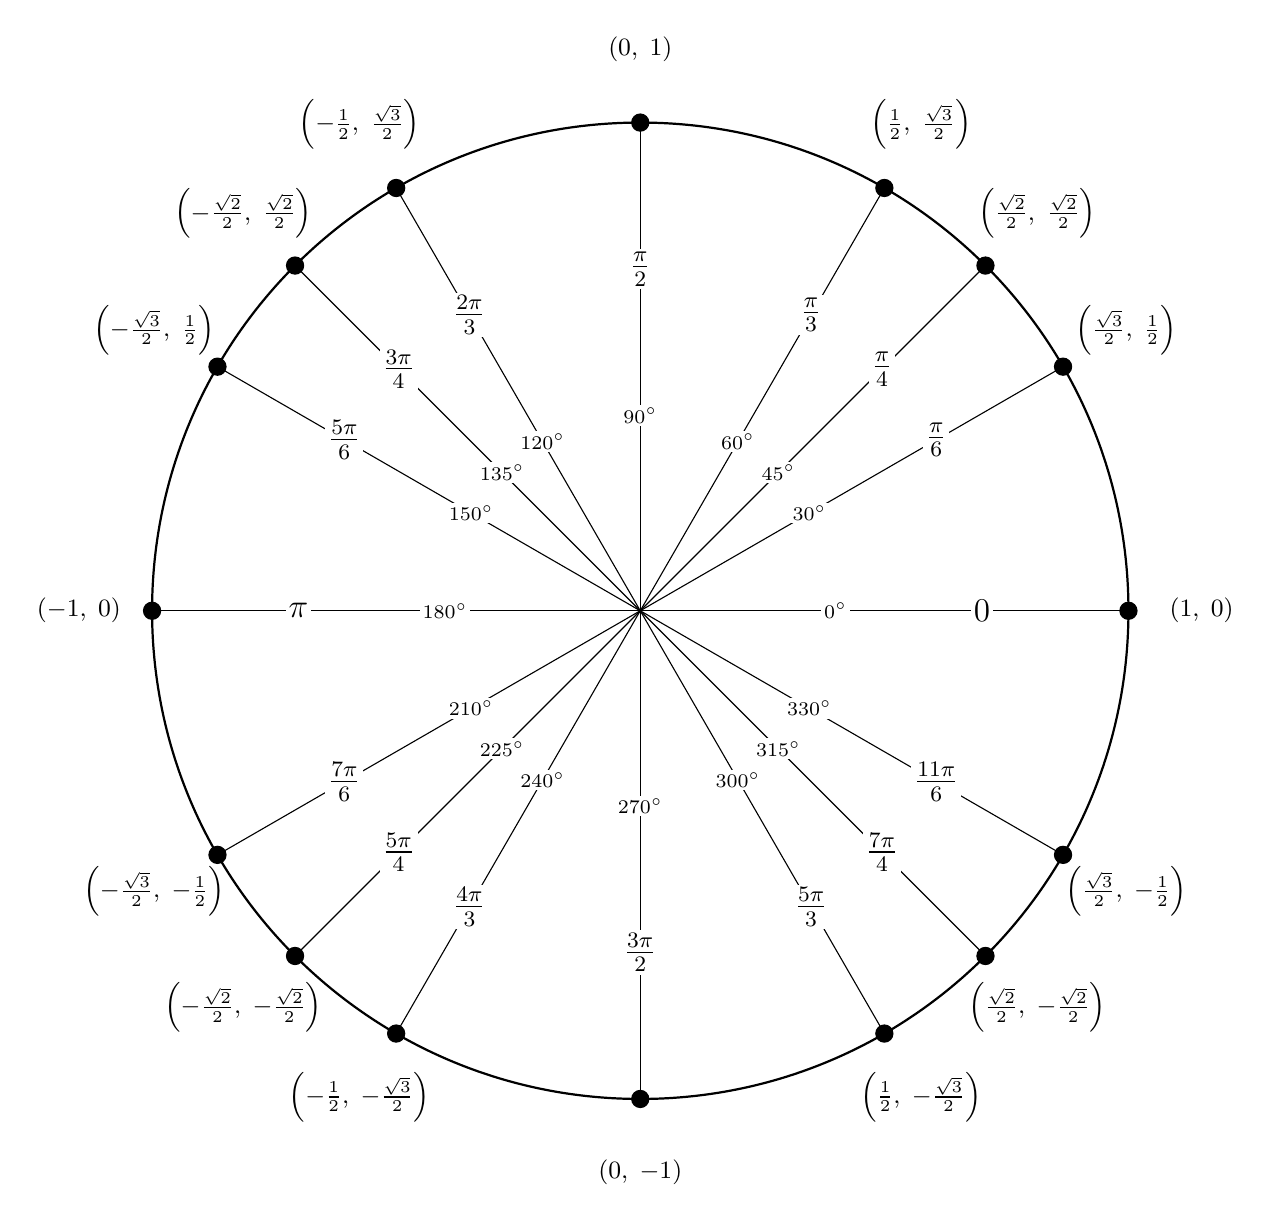
\begin{tikzpicture}[scale=6.2]
    % Unit circle
    \draw[thick] (0,0) circle (1cm);
    
    % All angles with their exact coordinates (including quadrantal angles)
    \foreach \angle/\rad/\cosval/\sinval in {
        0/0/1/0,
        30/\frac{\pi}{6}/\frac{\sqrt{3}}{2}/\frac{1}{2},
        45/\frac{\pi}{4}/\frac{\sqrt{2}}{2}/\frac{\sqrt{2}}{2},
        60/\frac{\pi}{3}/\frac{1}{2}/\frac{\sqrt{3}}{2},
        90/\frac{\pi}{2}/0/1,
        120/\frac{2\pi}{3}/-\frac{1}{2}/\frac{\sqrt{3}}{2},
        135/\frac{3\pi}{4}/-\frac{\sqrt{2}}{2}/\frac{\sqrt{2}}{2},
        150/\frac{5\pi}{6}/-\frac{\sqrt{3}}{2}/\frac{1}{2},
        180/\pi/-1/0,
        210/\frac{7\pi}{6}/-\frac{\sqrt{3}}{2}/-\frac{1}{2},
        225/\frac{5\pi}{4}/-\frac{\sqrt{2}}{2}/-\frac{\sqrt{2}}{2},
        240/\frac{4\pi}{3}/-\frac{1}{2}/-\frac{\sqrt{3}}{2},
        270/\frac{3\pi}{2}/0/-1,
        300/\frac{5\pi}{3}/\frac{1}{2}/-\frac{\sqrt{3}}{2},
        315/\frac{7\pi}{4}/\frac{\sqrt{2}}{2}/-\frac{\sqrt{2}}{2},
        330/\frac{11\pi}{6}/\frac{\sqrt{3}}{2}/-\frac{1}{2}
    }{
        % Draw line from origin to point on circle
        \draw[thin] (0,0) -- (\angle:1);
        
        % Point on circle
        \draw[fill=black] (\angle:1) circle (0.5pt);
        
        % Degree label inside circle (at 0.4 radius)
        \node[font=\scriptsize, inner sep=1pt, fill=white] at (\angle:0.4) 
            {$\angle^\circ$};
        
        % Radian label inside circle (at 0.7 radius)
        \node[font=\large, inner sep=1pt, fill=white] at (\angle:0.7) 
            {$\rad$};
        
        % Coordinate labels OUTSIDE circle (at 1.15 radius)
        \node[font=\small, align=center] at (\angle:1.15) 
            {$\left(\cosval,\;\sinval\right)$};
    }
    \end{tikzpicture}
\end{center}


\begin{table}[h!]
\centering
Sammenhæng mellem positive og negative radianer:
\label{tab:radian_relations}
\begin{tblr}{
    colspec = {*{17}{c}},
    vlines,
    row{1} = {mode=math},
    row{3} = {mode=math},
    row{2} = {mode=math},
    colsep = 4pt,   % horizontal space between columns
    rowsep = 4pt       % vertical space between rows
    }
    \hline
    0 & \frac{\pi}{6} & \frac{\pi}{4} & \frac{\pi}{3} & \frac{\pi}{2} & \frac{2\pi}{3} & \frac{3\pi}{4} & \frac{5\pi}{6} & \pi & \frac{7\pi}{6} & \frac{5\pi}{4} & \frac{4\pi}{3} & \frac{3\pi}{2} & \frac{5\pi}{3} & \frac{7\pi}{4} & \frac{11\pi}{6} & 2\pi \\
    \updownarrow & \updownarrow & \updownarrow & \updownarrow & \updownarrow & \updownarrow & \updownarrow & \updownarrow & \updownarrow & \updownarrow & \updownarrow & \updownarrow & \updownarrow & \updownarrow & \updownarrow & \updownarrow & \updownarrow \\
    -2\pi & \frac{-11\pi}{6} & \frac{-7\pi}{4} & \frac{-5\pi}{3} & \frac{-3\pi}{2} & \frac{-4\pi}{3} & \frac{-5\pi}{4} & \frac{-7\pi}{6} & -\pi & \frac{-5\pi}{6} & \frac{-3\pi}{4} & \frac{-2\pi}{3} & \frac{-\pi}{2} & \frac{-\pi}{3} & \frac{-\pi}{4} & \frac{-\pi}{6} & 0 \\
    \hline
\end{tblr}
\end{table}

\bemærkBig{%
    Radianer kan konverteres til grader ved at gange med \(\frac{180}{\pi}\) og grader kan konverteres til radianer ved at gange med \(\frac{\pi}{180}\).
}